%TODO: there should be some graph to demonstrate the last-mile problem.

In our baseline models, it is not very difficult to reduce the mean square error from millions to thousands. However, it is much harder to reduce it from thousands to tens. This is the so called last-mile problem.

In order to solve this problem, recursive model index was proposed \cite{kraska2018case}. The idea is to split the whole set of data into smaller pieces and assign each piece an index model. By doing so, each model is only responsible for a small range of keys. Ideally, in each smaller range, the keys are distributed in a way that is easier to be learned by our index models, such as polynomial model, fully connected model or even traditional B-Tree model.

As shown in Fig. \ref{rmi_structure}. A recursive model can be regarded as a tree structure, which contains a root model that receives the full dataset for training. Then the root model will split the dataset into several parts. Each sub-model will then receive one part of the full dataset. Then we train the sub-models one by one with the partial training dataset. 

\begin{mscexample}
	For example, in the Fig. \ref{rmi_structure}, the full dataset will be split into three parts and each sub-model receives one part. To train this recursive model, we first train the root model with the whole dataset. Then the root model will split the dataset into 3 parts according to the predicted value of each data point in the dataset. Then each sub-model will receive one part and we train the sub-model accordingly.
\end{mscexample}

\begin{figure*}[h]
\centering
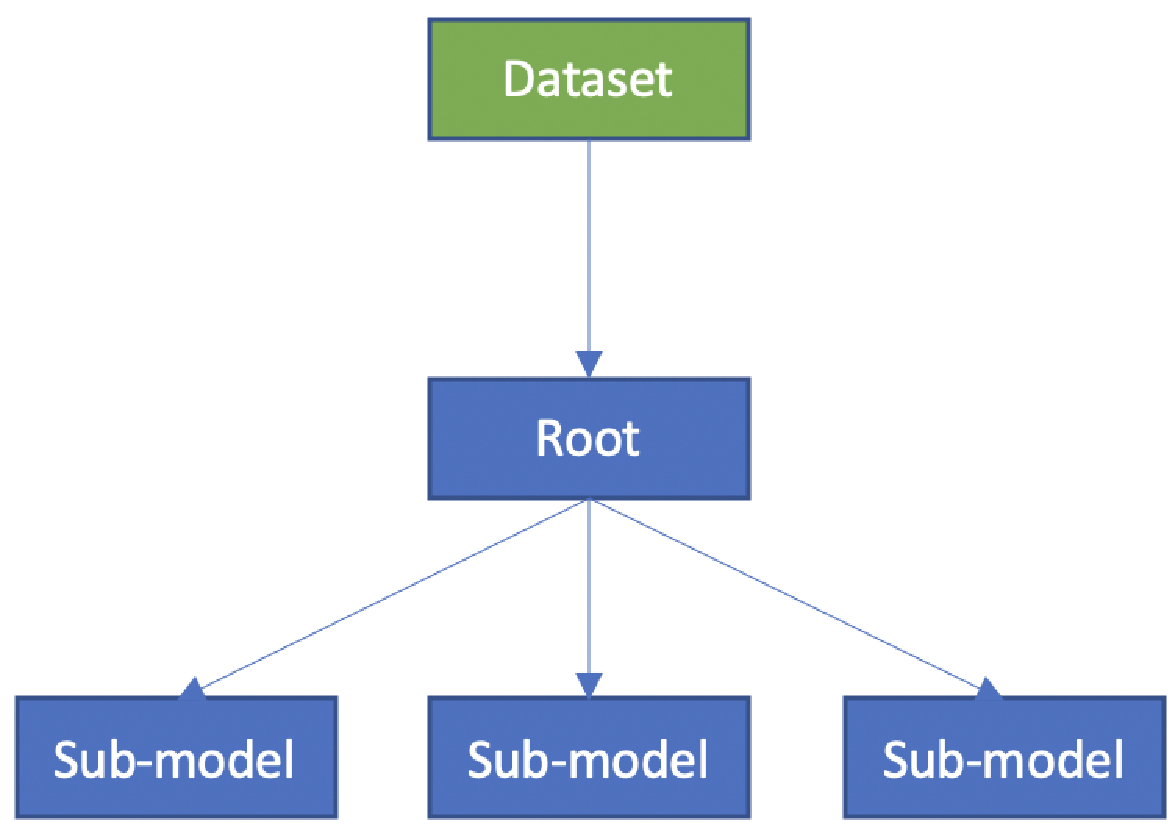
\includegraphics[scale=0.4]{graphs/rmi_demo}
\caption{An example recursive model index with one root model and three leaf model.}
\label{rmi_structure}
\end{figure*}



\subsubsection{Definitions}

Similar to a tree, we define the following terms in a recursive model:

\begin{enumerate}
	\item \textbf{Node Model}. Every node is responsible for making decisions with given input data. In one dimensional case, it can be regarded as a function $f:\mathbb{R}\to\mathbb{R}, x\to y$ where $x$ is the input index and $y$ is the corresponding page block. In principle, each node can be implemented as any machine learning model, from linear regression to neural network, or a traditional tree-based model, such as B-Tree.
	\item \textbf{Internal Node Model}. Internal nodes are all nodes except for leaf nodes and the root node. Every internal node receives a certain part of training data from the full dataset, and train a model on it. 
\end{enumerate}

In the following sections, we will use the notations defined below:
\begin{enumerate}
	\item $N_M^{(i)}$ is the number of models in the $i$th stage.
	%TODO: more notations
	%TODO: modify algorithms accordingly
\end{enumerate}


\subsubsection{Training}

In order to construct a recursive model, we need to have several parameters listed below:
\begin{enumerate}
	\item The training dataset, notated as $(X, Y)$ with entries notated as $(x,y)$.
	\item The number of stages, notated as $N_S$. It is an integer variable.
	\item The number of models at each stage, notated as $N_M$. It is a list of integer variable. $N_M^{(i+1)}$ represents the number of models in the $i$th stage.
\end{enumerate}

The training process of recursive model is an up-bottom process. There will be only one root model that receives the whole training data. After the root model is trained, we iterate over all the training data and predict the page by the root model. After the iteration, we get a new set of pairs $(X, Y_0)$. Then we map $\forall y_0\in Y_0$ into the selected model id in next stage by $\texttt{next}=y_0 * N_M^{(i+1)}/\texttt{max(Y)}$.

\begin{algorithm}[H]
    \SetAlgoLined
    \SetKwInOut{Input}{input}
    \Input{\texttt{num\_of\_stages; num\_of\_models; types\_of\_models; x; y}}
     \texttt{trainset=[[(x,y)]]} \\
     \texttt{stage$\gets 0$} \\
     \While{\texttt{stage} \textless \texttt{num\_of\_stages}}{
      \While{\texttt{model} \textless \texttt{num\_of\_models[stage]}} {
        \texttt{model.train(trainset[stage][model])} \\
        \texttt{models[stage].append(model)}
      }
      \uIf{not last stage} {
        \For{$i\gets0$ \KwTo $len(x)$}{
            	\texttt{model=models[output from previous stage]} \\
            	\texttt{output=model.predict(x[i])} \\
            	\texttt{next=output * num\_of\_models[stage+1]/max\_y} \\
            	\texttt{trainset[stage+1][next].add((x[i],y[i]))}
        }
      }
     }
     \caption{Training of Recursive Model Index}
\end{algorithm}

\subsubsection{Prediction}

\begin{algorithm}[H]
    \SetAlgoLined
    \SetKwInOut{Input}{input}
    \Input{\texttt{x; models; num\_of\_stages; max\_y}}
     \texttt{stage$\gets 0$} \\
 	 \texttt{next\_model$\gets 0$} \\
     \While{\texttt{stage} \textless \texttt{num\_of\_stages}}{
        \texttt{output = model.predict(x)} \\
        \texttt{next\_model=output*len(models[stage+1])/max\_y}\\ 
      \uIf{last stage} {
		\texttt{y = next}
      }
     }
     \caption{Training of Recursive Model Index}
\end{algorithm}
